\documentclass[conference]{IEEEtran}

\usepackage{url}
\usepackage{multirow}
\usepackage{array}
\usepackage{epsfig}
\usepackage{footnote}
\usepackage{amsmath}

\widowpenalty=100000
\clubpenalty=100000

\begin{document}

\title{Grid Appliance -- On the Design of Self-Organizing,
Decentralized Grids}

\author{
\IEEEauthorblockA{
  David Isaac Wolinsky,
  Arjun Prakash,
  Renato Figueiredo
}
\IEEEauthorblockN{
  University of Florida
}
}

\maketitle


\begin{abstract}

``Give a man a fish, feed him for a day.  Teach a man to fish, feed him for a
lifetime'' -- Lau Tzu

Grid computing projects such as TeraGrid~\cite{teragrid},
Grid'5000~\cite{grid_5000}, and OpenScience Grid~\cite{osg} provide researchers
access to vast amounts of compute resources, but in doing so, require the
adaption of their workloads to the environments provided by these systems.
Researchers do not have many alternatives as creating these types of systems
involve coordination of distributed systems and expertise in networking,
operating systems, security, and grid middleware.  This results in many
research groups creating small, in-house compute clusters where scheduling is
often ad-hoc, thus limiting effective resource utilization.  To address these
challenges we present the ``Grid Appliance.''  The ``Grid Appliance'' enables
researchers to seamlessly deploy, extend, and share their systems both locally
and across network domains for both small and large scale computing grids.
This paper details the design of the Grid Appliance and reports on experiences
and lessons learned over four years of development and deployment involving
wide-area grids.

\end{abstract}

\section{Introduction}

Grid computing presents opportunities to combine various scale, distributed
resources together to form powerful computing systems.  Due to the challenges
in coordinating the organization of grids, researchers typically become members
of existing grids or often times inefficently manage their local resources,
such as resource discovery and allocation by word of mouth.  While there is a
wealth of grid middleware available, including resource managers like
Condor~\cite{condor0}, Torque (PBS)~\cite{torque}, and Sun Grid
Engine~\cite{grid_engine} and parallelization tools like MPICH~\cite{mpich},
Hadoop~\cite{hadoop}, and UPC~\cite{upc}, most researchers see the entry
barrier to installing and future management of the system as being greater than
their usefulness.  To address these concerns, we have implemented the ``Grid
Appliance'' allowing users to focus on making use of the grid and not the setup
and management of the underlying components.

At the heart of our approach lies a P2P infrastructure enabling decentralized
peer discovery thus coordinating the organization of a grid.  The chosen P2P
infrastructure is based upon distributed hash tables (DHTs) enabling peers to
efficiently query the system with a key and potentially receive multiple values
without complex searching algorithms.  To address wide area connectivity and
network dynamics, we employ a virtual private network (VPN), guaranteeing
all-to-all connectivity while transparently handling configuration and
organization through the DHT.  Grid configuration happens automatically through
web interface configuration files and node interaction through the DHT or VPN
based IP multicast.  The entire system has been packaged into a software
repository enabling automatic configuration of physical, virtual, and even
cloud resources.  This results in the ``Grid Appliance'', a preconfigured
environment emphasizing user-centricity and trivial installation.  This
approach focuses user interaction with the system on their tasks rather than
the configuration details, providing researchers with a plug-and-play tool to
create ad-hoc virtual compute clusters for their own groups, local or
federated.  

The web interface used to create the appliance configuration is called ``Group
Appliances.'' At this site, users create or join groups, similar to an online
social networking group.  Administrators of the group have the abilities to
accept or deny user access and remove misbehaving users.  All members of the
group have the ability to create and download configuration files, which plug
into the ``Grid Appliance'' as a floppy disk or as a file in its file system.
The file specifies the type and purpose of the ``Grid Appliance'' instance and
uniquely identifies the owner.  Upon first boot, an appliance instance contacts
the ``Group Appliances'' site specified in the configuration file to obtain a
certificate authority (CA) signed certificate, after which the system becomes
completely decentralized and connects to other systems through the P2P overlay.  

To justify our techniques, consider the difficulty in combining resources
across disparate networks, which may or may not involve multiple research
groups.  Challenges such as safety, security, connectivity, and efficiency may
require an information technology (IT) expert.  Network constraints present
another complexity beyond configuration and organization of distributed
resources.  Contributing groups may have resources behind different network
address translators (NATs) and firewalls, preventing direct communication with
each other.  Even assuming that an institution's network administrator is
willing to make exceptions for the grid, additional rules may be required for
each new cluster or resource added internally and externally, quickly becoming
unmanageable.  Our system embraces these concerns, we assume a completely
decentralized system with many if not all resources behind NATs, that users may
be unfamiliar with networking considerations and managing grid organization;
but the system still works well when used inside a LAN controlled by
experienced IT workers.

The rest of this paper discusses these challenges in more depth and our
solutions addressing them.  In Section~\ref{middleware}, we discuss various
types of middleware and techniques used to support self-configuration.
Section~\ref{vpns} reflects on the difficulties presented by distributed
systems and how only a small subset of VPNs can provide a satisfactory
solution.  The entire architecture of the system is presented in
Section~\ref{system}.  Finally, Section~\ref{related_work} compares and
contrasts other solutions to these problems.

\section{Middleware}
\label{middleware}

We consider two types of grid middleware in this paper:  resource management /
batch task systems and application specific tools.  Resource management systems
like Torque, Condor, and Sun Grid Engine (SGE) consist of three fundamental
components: execute nodes, resource managers, and submission nodes.  The
execute nodes run the tasks submitted from the submission sites.  Users access
a submission site, craft task description files, and submit them to a scheduler
or resource manager, which will queue tasks to the various execute nodes.
Application specific systems like Hadoop, MPICH, and UPC do not have such a
convenient layout, but typically all-to-all connectivity is required amongst
the resources.

A user configuring grid middleware must understand the layout of the system,
install the correct software on each resource, and then configure all the
individual resources to work with each other.  Use of packaging as described in
Section~\ref{system} addresses the concerns of software.  While the
configuration data, users download from the ``Group Appliances,'' determines
how to configure the individual resources.  This section addresses
decentralized resource configuration.  Without it, users would, potentially,
need to communicate with each other each time new resources were added,
removed, or there was some system change, like an IP address changing.  We
explore the usage of both DHT and IP multicasting to allow users to forego this
configuration issue.

\subsection{Resource Managers and the DHT Approach}

The first goal of the ``Grid Appliance'' is to construct wide area grids using
common resource management techniques.  To do so efficiently, we employ the
DHT.  In this manner, a manager places its IP address into the DHT at the key
\emph{managers}.  When workers and clients join the grid, the systems
automatically query this key and configure to report to one or more managers,
application dependent.  Likewise, managers can query this key and then
coordinate with each other management of the overlay.

Of the resource management middlewares that we have surveyed, Condor was the
most appealing due to its decentralized properties and focus on desktop grids.
These are easily recognizable by analyzing the complexity involved in having
multiple submission sites and the ability to add and remove resources.

Typical clusters have a single entry point for task submission, SGE and Torque
make it rather difficult to support more than one, usually requiring additional
middleware, such as Globus~\cite{globus}, to support this behavior.  If
multiple groups are collaborating together to form a single grid, a single
submission site may be very undesirable and difficult to support.  To allow for
multiple submission sites, Condor separates job queues / submission sites from
resource management and so that two entities work together to negotiate the
running jobs on resources.  In our system, job queue or submission machine,
which stores everything pertinent to the user, is run by the user, while the
resource manager runs independently with Condor handling all the interaction
between it and the job queue.

To add new resources to a Condor system, an execute or submission node must
have an IP address for the manager, the rest of the system organization is
performed entirely transparent to the user.  However, in SGE and Torque, after
resources have been added into the system, the user must manually configure the
manager to control them.

One of the caveats of our approach, which remains ongoing research, is the
requirement of a manager, which means we do not provide a completely
decentralized, but rather a distributed approach.  In the meantime, we have
taken advantage of a feature known as ``flocking'' in Condor.  Flocking allows
submission sites to connect to multiple managers.  This serves two purposes: 1)
to provide transparent reliability by supporting multiple managers and 2) users
can share their resources through their own manager.

To configure Condor, we store managers IP addresses into the DHT using the key
\emph{managers}.  When a new peer joins, it queries the DHT, obtains the list
of all managers, and randomly selects one as its primary manager.  The rest are
set to flocking.  If the system prefers managers from its group, it will
randomly contact each manager in an attempt to find a match, selecting one at
random if no match is found.  If no managers are found, the process repeats
every 60 seconds.  Once a manager has been found, it is checked every 10
minutes to ensure it is online and additional managers that have come online
are added to the flock list.

\subsection{Hadoop, MPICH, and Multicast Discovery}

Alternatively users may want to experiment with tools meant for LANs but not
want to invest the time to install and configure them.  In which case, DHT use
does not translate well if they want to install software without using our
appliance domain.  To support these endeavours, we have investigated methods to
bootstrap grid middleware through IP multicast.  IP multicast works on all LANs
and is used by many popular applications for discovery, such as Windows Media
Center and iTunes by meanas of the UPNP (DLNA) and DAAP protocols,
respectively.

\begin{figure*}[h!t!]
\centering
\epsfig{file=figs/NAT.eps, width=5in}
\caption{A typical NAT interaction. The peer behind a NAT has a private address.
When the packet is sent through the NAT, the NAT translates the source information
into a public mapping, keeping the original source information so that if a
packet from the remote peer comes back, it can be translated and delivered to
the original source.}
\label{fig:nat}
\end{figure*}

The two systems that we have used to configure through IP multicast are Hadoop
and MPICH.  Hadoop configuration consists of a head node and worker nodes,
where the head node distributes map tasks to the worker nodes.  In MPICH, each
resource is identically configured to support interprocess communication
through the MPICH library, it is up to the application developer to determine
roles of individual nodes.  In both cases, the way multicast discovery works is
to send out a beacon requesting that all nodes supporting these services
respond.

Our appliance setup for these applications consists of a common ssh key, so
that all resources in a grid can connect with each other and a multicast
discovery application so a coordinator can organize the resources.  The ssh key
only enables access on host only networks and VPNs, preventing malicious
third-parties from gaining access to the grids.  The IP multicast script is run
by the user on a single access node, which will act as the coordinator.  The
resource discovery sends out a beacon several times and after a 30 second
delay, the process completes and all responding resources are automatically
configured through ssh.

\section{The Motivation for VPNs}
\label{vpns}

As of 2010, the majority of the Internet is connected via Internet Protocol
(IP) version 4.  This protocol has a quickly approached limit of addresses
available,  only $2^{32}$ (approximately 4 billion).  With the Earth's
population at over 6.8 billion and each individual potentially having multiple
devices with Internet connectivity, the IPv4 limitation is becoming more and
more apparent.  Addressing this issue are two approaches:  1) the use of NATs
to enable many machines and devices to share a single IP address but preventing
bidirectional connection initiation, and 2) IPv6 which supports $2^{128}$
addresses.  The use of NATs, as shown in Figure~\ref{fig:nat}, complicates grid
systems that require all-to-all communication, which include all of those which
we consider.  In addition, firewalls may prevent peers from receiving incoming
connections.  And while the eventual widespread use IPv6 may eliminate the need
for address translation, it does not deal with the issue of firewalls, and the
future of NATs in IPv6 is unclear.

VPNs motivate from more than just crossing NATs and firewalls.  With a VPN,
users can avoid the headaches associated with dynamic IP addresses, as each
resource can claim an IP and, regardless of the machines physical location, use
it, an ideal condition for laptop users.  In addition, it abstracts the user
from having to be concerned about network addresses.  The mixture of virtual
machine NATs and VPNs allow users inside a network to not be concerned about IP
address allocations, from the LANs perspective, the machine has only ever been
allocated one IP address, yet all grid resources are able to communicate with
each other.

Our work relies on a group enabled IPOP VPN called GroupVPN~\cite{groupvpn}.
IPOP through its underlying P2P infrastructure support NAT traversal allowing
for peers behind NATs to communicate directly with each other in addition to
indirectly communicating by relaying across the P2P system.  Many of the key
features of our grid system are enabled because of the VPN.  For example, if
there were not a VPN, users of MPI and Hadoop would need to ensure that all
resources were bridged to the LAN and not through a VM NAT, the typical
configuration, otherwise the multicast message would not be delivered to all
participants.  The VPN software supports the ability to self-organize using
existing infrastructures including IP multicast, public overlays, and Xmpp as
described in our previous work~\cite{p2p10}.  This is in contrast to other VPNs
that are either centralized and require a dedicated node to coordinate peers
and decentralized solutions that require manual configuration of links between
peers.

\begin{figure*}[ht]
\centering
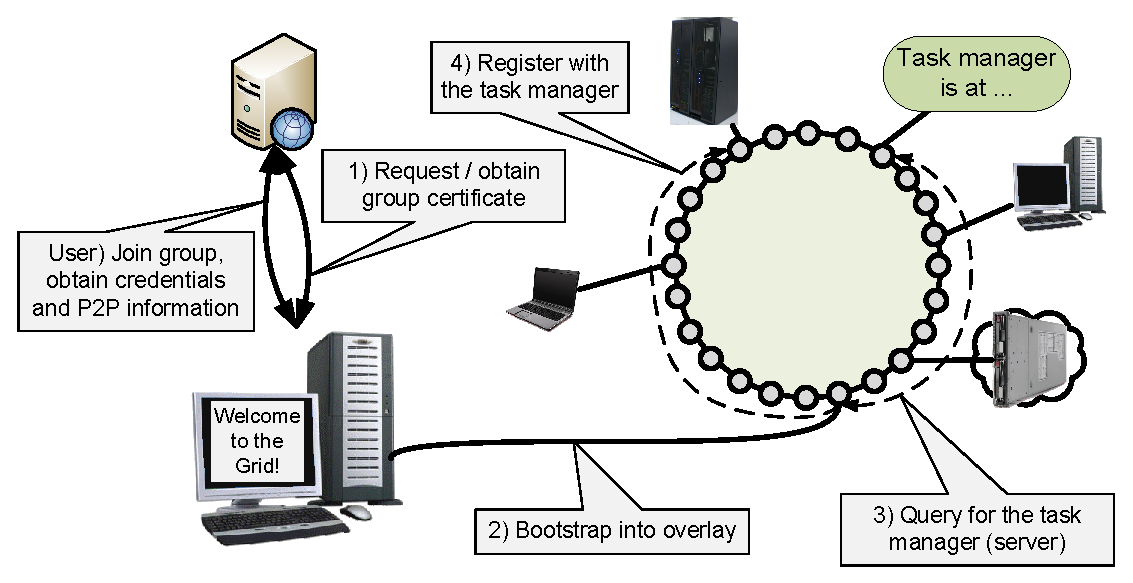
\epsfig{file=figs/system.eps, width=6in}
\caption{An example deployment scenario:  obtaining configuration files, to
starting the appliance, and connecting with a resource manager.}
\label{fig:system}
\end{figure*}

Using these techniques ``Grid Appliances'' can be constructed in one of two
ways: local and wide area.  The ``Grid Appliance'' ships with two default
configurations, one that connects users to a globally available public system
and another that allows for LAN only grids.  Local grids can be constructed by
booting the appliances, which will then use multicast self-discovery to find
other resources, create the DHT overlay, and then form VPN links.
Alternatively, the user can connect to the default publc system or use ``Group
Appliances'' to create and manage their own grid, both of which bootstrap from
a public shared DHT overlay.  This does not prohibit more advanced users from
downloading our ``Group Appliances,'' as its available as a VM, and host their
own DHT overlay.

\section{Deploying Grid Appliances}
\label{system}

The complete system is presented in Figure~\ref{fig:system}.  Users join a
group and can then download one of three different types of configurations:
server, worker, and client (mapping to the three types of typical grid nodes,
resource manager, execution site, and submission site).  In addition to the
configuration data, a first time user can download the generic appliance, or
one extended with additional software customized for their community.  In the
case of a VM appliance, the configuration data can be added to the system as a
virtual floppy image, automatically configuring the appliance for a specific
behavior.  In the case of the client, it begins searching for an appropriate
resource manager by querying the DHT.  Upon finding an entry in the DHT, the
client communicates with the resource manager via the VPN.  The same procedure
can be repeated many times to add additional resources into the grid.
Resources booted using the ``server'' image configure and advertise themselves
through the DHT or VPN.  Each individual grid can support multiple servers for
fail-over or load balancing, depending on the capabilities of the grid
middleware (e.g. Condor flocking).  Beyond the downloading of the appliance and
the configuration data, all other steps are performed transparently from the
user.

VMs are favored for the distribution of complicated applications as experts can
configure them and release the results as a complete working system.  This
approach may limit non-expert use to the VM appliance, which may be undesirable
for users that want to configure their own systems without reuse of the
existing VM.  Guides may exist for the creation of systems, most systems are
too complex for non-experts to produce similar results found in the VM.  In
addition to supplying VMs, we also supply packages for Debian and Ubuntu
systems, DEB files.  These enable easy installation in arbitrary environments
through the use of package managers, APT in the case of Debian and Ubuntu,
which handle configuration and dependencies, allowing users can focus on the
end result and not stumbling during setup.  Given an Ubuntu or Debian
installation on a physical, virtual, or cloud machine, a new ``Grid Appliance''
can be configured by following these steps:  add the configuration data into
the newly configured resource, our package repository to the remote
repositories list, and our repositories signing key to the key chain for
repositories and finally selecting our packages and installing them.  At which
point, the system will connect to the grid.

To verify the utility of our approach, we have evaluated the time required to
create and utilize a grid consisting of various distributed resources using the
``Grid Appliance.'' The system consists of VMware resources behind a Cisco and
``iptables'' NAT at the University of Florida (UF), KVM resources behind an
``iptables'' and KVM NAT at Northeastern University (NEU), and cloud resources
provided by Amazon's EC2, pools of 50 resources from each site were booted
independently and then together, resulting in 4 different test runs.

Each test was performed independently with an existing manager and submit node
already in the system.  We measure three times during this evaluation:
``start'' - begins with starting the experiment including the copying of files
and creation of instances until all resources have been powered on, ``connect''
- is the time delta between the end of ``start'' and when all resources appear
in ``condor\_status,'' that is, have registered with the manager, and ``run'' -
time from the submission to the conclusion of a 5 minute job to all resources
Like connect, run measures the time for VPN connections, only from the client
to the resources instead of from the negotiator.  All tasks are automated
through scripts with human interaction required only to start the events of
grid boot and job submission.  Results are presented in
Figure~\ref{fig:results}.

\begin{figure}[ht]
\small{
\setlength{\itemsep}{0pt}
\setlength{\parskip}{0pt}
\centering
\begin{tabular}[c]{|m{1.0cm}||m{1.2cm}|m{1.3cm}|m{1.2cm}|m{1.2cm}|} \hline
& 50 - EC2 & 50 - NEU & 50 - UF & 150 - All \\ \hline\hline
Start & 2:44 & 10:21 & 20:23 & 21:14 \\ \hline
Connect & 2:27 & 11:36 & 3:53 & 17:13\\ \hline
Run & 7:15 & 6:35 & 5:53 & 21.19 \\ \hline
\end{tabular}
\caption{\small{Time in minutes:seconds to start and connect execute nodes from
various sites, Amazon EC2, Northeastern University, and University of Florida,
to an already online resource manager, and then the time to run a 5 minute job
from a freshly connected submission node.}}
\label{fig:results}
}
\end{figure}

As the systems consist of various hardware and software configurations, the
time to start is only provided as a reference to potential overheads in
bootstrapping the resources.  Some of the interesting experiences of the
experiment were:  1) the combination of the ``iptables'' and VMware NAT was
more easily traversable than the combination of ``iptables'' and KVM NAT and 2)
in the experiment consisting of 150 peers, nodes were actually well connected
much earlier, but due to missed packets and Condor timeouts, not all resources
were accounted for in Condor as early as in the other tests.  With regards to
the KVM NAT, it appears to be particularly aggressive as NAT mappings last for
less than 10 seconds, while typical NATs keep mappings for over 30 seconds.

\section{Related Work}
\label{related_work}

Existing work that falls under the general area of desktop grids/opportunistic
computing include Boinc~\cite{boinc}, BonjourGrid~\cite{bonjourgrid}, and
PVC~\cite{pvc}.  Boinc, used by many ``@home'' solutions, focuses on adding
execute nodes easy; however, job submission and management rely on
centralization and all tasks must use the Boinc APIs.  BonjourGrid removes the
need for centralization through the use of multicast resource discovery; the
need for which limits its applicability to local area networks.  PVC enables
distributed, wide-area systems with decentralized job submission and execution
through the use of VPNs, but relies on centralized VPN and resource management.

Each approach addresses a unique challenge in grid computing, but none
addresses the challenge presented as a whole: easily constructing distributed,
cross-domain grids.  Challenges that we consider in the design of our system
are ensuring that submission sites can exist any where not being confined to
complex configuration or highly available, centralized locations; ability to
dynamically add and remove resources by starting and stopping an appliance; and
the ability for individual sites to share a common server or to have one or
more per site so that no group in the grid is dependent on another.  We
emphasize these points, while still retaining the ease of use of Boinc, the
connectivity of PVC, and the flexibility of BonjourGrid.  The end result is a
system similar in organization to OurGrid~\cite{ourgrid}, though whereas OurGrid
requires manual configuration amongst sites and networking considerations to
ensure communication amongst sites, the ``Grid Appliance'' transparently handles
configuration and organization issues with a VPN to transparently handle network
constraints.

\section{Conclusions}
\label{conclusions}

In this paper, we have described a novel grid architecture that enables both
wide area and educational grid middleware.  Our results from
Section~\ref{system} show that the process of connecting the resources together
are not significantly longer than that of actually starting the resources.
Furthermore, we have shown that submission sites have very low overheads in
connecting to the resources.  For future work, we intend on expanding the
utility of the ``Grid Appliance'' to support completely decentralized grid
computing.

With regards to practical experience, we have been providing a service called
Archer~\cite{archer}, an active grid deployed for computer architecture
research, for nearly 3 years.  Archer currently spans four seed universities
with 500 resources with over hundreds of students and researchers submitting
jobs totaling over 150,000 hours of job execution in the past year alone.
Groups at the Universities of Florida, Clemson, Arkansas, and Northwestern
Switzerland have used it as a tool to teach grid computing.  Clemson and Purdue
are constructing campus grids using the underlying VPN to connect resources
together.  Recently, two private small-scale systems have come online using our
shared system available at \url{www.grid-appliance.org}.  Feedback from users
through surveys have shown that non-expert users are able to connect to our
public Grid appliance pool in a matter of minutes by simply downloading and
booting a plug-and-play VM image that is portable across VMware, VirtualBox,
and KVM.

\section*{Acknowledgments}

We thank the anonymous reviewers for their useful comments and feedback and
Perhaad Mistry for his help in providing direct access to Northeastern
University's Archer resources for experiments.  This work is sponsored by the
National Science Foundation under awards 0751112 and 0721867.  Any opinions,
findings and conclusions or recommendations expressed in this material are
those of the authors and do not necessarily reflect the views of the NSF.

\bibliographystyle{IEEEtran}
\bibliography{DecentralizedGrids}

\end{document}
